\subsection{Lavoro}

\textbf{Nota bene: } il lavoro($F$) è energia trasferita ad un corpo mediante le forze che agiscono su di esso. \\
\begin{center}
    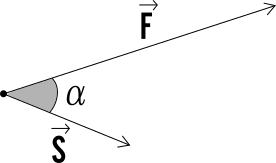
\includegraphics[width=0.4 \linewidth]{Dinamica/Lavoro/il-lavoro-di-una-forza.png}    
\end{center}
\begin{gather*}
    \textbf{Lavoro: } L = \vec{F} \cdot \vec{s} = F \cdot  s
\end{gather*}

\subsection{Lavoro della forza peso}

\begin{gather*}
    \textbf{Lavoro: } L = -mg(y_{finale} - y_{iniziale})
\end{gather*}

\subsection{Lavoro della forza elastica}

\begin{gather*}
    \textbf{Lavoro: } L = - \frac{1}{2} k (x_f^2 - x_i^2) \\
    \textbf{Elongazione iniziale: } x_i = L_i - L_0 \\
    \textbf{Elongazione finale: } x_f = L_f - L_0
\end{gather*}

\textbf{Nota bene: } nel caso di una molla a riposo($x_i = 0$)il lavoro($L$) sarà sempre negativo, che la molla venga compressa($x_f < 0$) o che venga allungata($x_f > 0$), poiché la forza elastica della molla resiste all'elongazione.

\begin{gather*}
    \textbf{Molla compressa: } x_f < 0 \\
    \textbf{Molla allungata: } x_f > 0 \\
    \textbf{Lavoro: } L = - \frac{1}{2} k (x_f^2)
\end{gather*}